\section{Methodology}

The proposed methodology can be summed in three main parts. 
The first step is audio preprocessing, we than add data augmentation, 
and lastly feature extraction.

The dataset picked for the study is the Ryerson Audio-Visual Database of Emotional Speech
and Song (RAVDESS). For the purpose of the project only speech audio files are 
considered.
Data is divided among 24 actors and 8 different emotions are present, namely: 
neutral, calm, happy, sad, angry, fearful, disgust and surprised.
Figure \ref{fig:classes} shows the classes distribution, we can see some imbalance. 
Data imbalance needs to be fixed during training, as a classifier could achieve an high accuracy 
score having terrible performance on underrepresented classes. 

There are many ways to tackle the problem, one is to augment the underrepresented classes, another 
one is to trim the dataset to have equal data distribution, and the last one is to use class weights 
during training. This last one is going to be the selected approach, it consists in multiplying 
the error on some classes by a factor, that takes into consideration the lower cardinality of 
some labels.  


\begin{figure}
  \begin{center}
      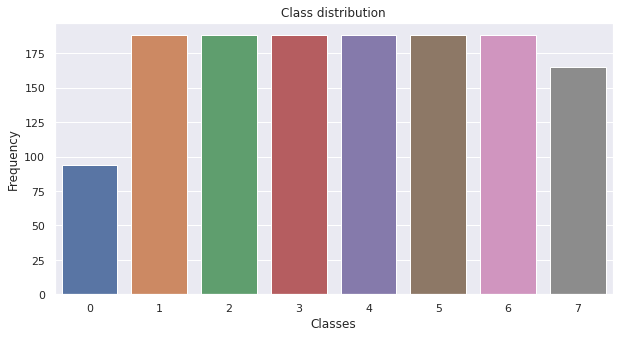
\includegraphics[width=0.7\textwidth]{images/classes.png}
      \caption{Dataset classes distribution.} \label{fig:classes}
  \end{center}
\end{figure}

\subsection{Feature extraction}

Before extracting features, we pad all audio files to the same length, 
that is the max of all the dataset. 
This is to avoid differences in dimensionality in later phases. The overall 
dataset duration distribution can be seen in Figure \ref{fig:dur}.

\begin{figure}
  \begin{center}
    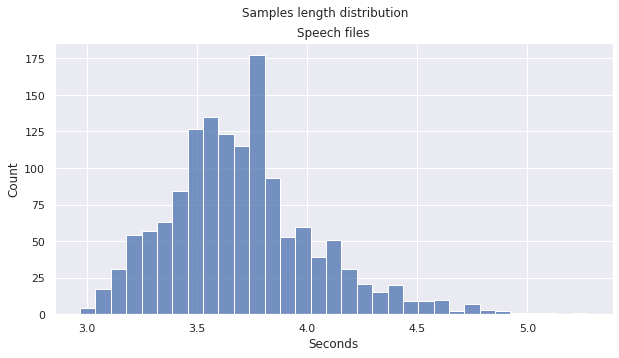
\includegraphics[width=0.7\textwidth]{images/duration.png}
    \caption{Audio duration distribution on the dataset.} \label{fig:dur}
  \end{center}
\end{figure}

\noindent After padding all the audio files to the same length, feature
extraction can take place.
The selected features are:
\begin{itemize}
  \item Pitches: pitches are extracted from the 
  files, we then can compute mean, std, max and min. Also, the pitch tuning offset is computed;
  \item Spectral centroid: after computing the spectral centroid, we normalize it
  and consider the mean, std and max;
  \item Flatness: another feature is the mean of the spectral flatness;
  \item MFCC: the first 50 mfcc are extracted and transposed. We then can consider
  the mean, std and max for each vector.
  \item Root-mean-square: the mean, max and std of the root-mean-square is computed.
\end{itemize} 
Finally, the mean of chromagram, melspectrogram, spectral contrast and zero crossing rate 
are considered.
A total of 312 features are obtained for each audio file. 

\noindent Figure \ref{fig:2d} shows a two-dimensional projection of the dataset, 
obtained using Principal component analysis on the extracted features, with the labels associated by K means.
K is set to $3$, found with the elbow method. The figure shows the difficulty of the task, indeed the 
we can see that clusters 0 and 1 have a great amount of labels associated with them, hence no 
real separation is present in the feature space.

\begin{figure}
  \begin{center}
    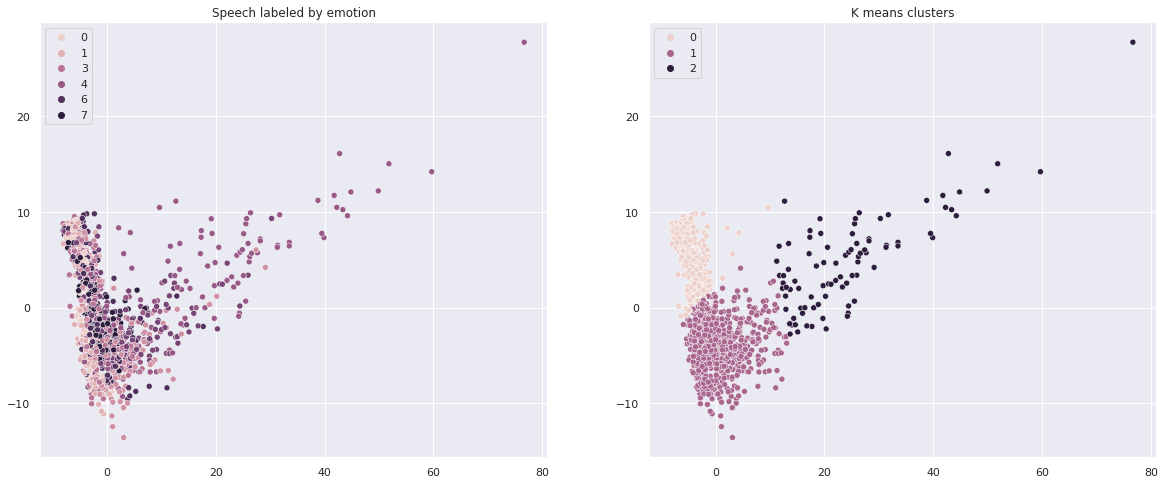
\includegraphics[width=\textwidth]{images/2d.png}
    \caption{Two-dimensional projection and K-means clusters of the extracted features.} \label{fig:2d}
  \end{center}
\end{figure}

\noindent After extracting features, they are scaled to have unit variance and 
zero mean. 
Also, Principal component analysis is an option, as it reduces dimensionality by 
keeping almost all the original variance of the data, the study on this 
part has been removed from the report as the performance is much worse with respect 
to keeping all the 312 features.

To train the Convolutional neural network, only the MFCC is uses, extracted in the same way 
discussed above.

\subsection{Data augmentation}

To avoid overfitting of the training set and potentially increase 
performances on the test set, a data augmentation phase is employed.
The goal is to increase the number of samples to help models with generalization. 
A raw audio is considered and a transformation is picked, the latter is parametrized to 
regulate the intensity of the change. 

\noindent The tree transformations used in the project are: 
\begin{itemize}
  \item Speed: audio is speed up or slowed down randomly. The ratio 
  in speed change goes from 0.6 to 1.4;
  \item Pitch: the pitch is shifted up or down randomly between -4 and +4 semitones;
  \item Noise: gaussian noise is added, the amplitude ranges from 0.0005 to 0.002.
\end{itemize}

\noindent Every augmenter is applied on the whole dataset, resulting 
is a cardinality that is four times the original.
Note that data augmentation happens only on the training split, the test one is 
always left untouched. 
An example of data augmentation can be seen in Figure \ref{fig:aug}. 

\begin{figure}[H]
  \begin{center}
    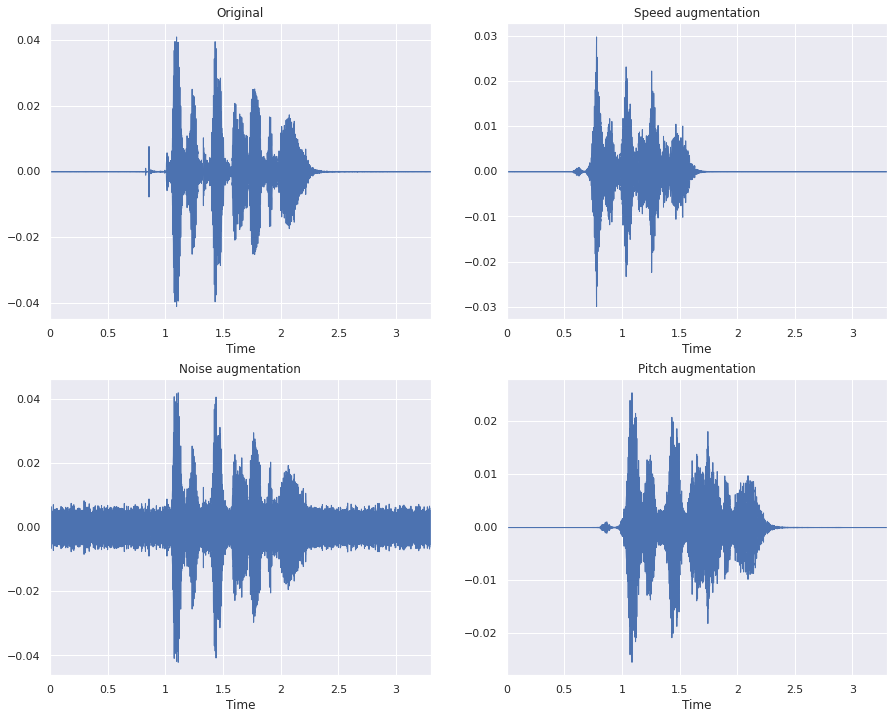
\includegraphics[width=0.9\textwidth]{images/aug.png}
    \caption{Data augmentation effects on example audio file.} \label{fig:aug}
  \end{center}
\end{figure}

\noindent One of the key factors when augmenting data is to keep the augmented samples plausible. 
Indeed, too much data augmentation result in training samples that do not help with generalization, 
while too little simply duplicates data in the training set.
The augmentation ranges are selected in an empirical way, after various tries. 

\section{Models definition}

The section talks about the models used in the study. 
We first start with classical ones and then focus on neural networks 
architectures.

\subsection{Classical models}
The classic models used are Support Vector Machines, K-NN and Decision trees.
The first one is left at default parameters, so the kernel is the radial basis function, 
regularization is set to one, gamma is set to scale. 
The choice of K for the nearest neighbors classifier is $\sqrt{|X|}$ where $X$ is the training set.
Lastly, the max number of levels of the decision tree is set to 10 to avoid 
over-fitting the data.

\subsection{Neural network}

A multilayer perceptron is used on the 312 features dataset. 
The architecture is quite simple at only four layers.
The first layer has 128 neurons, the second 64, the third 32 and lastly 8 
neurons for classification. 
All activation functions are relu, apart from the last that uses 
a softmax.
The Dense layers are separated by Dropouts with probability of 0.3.

The loss is the Sparse Categorical Cross-entropy, while the 
optimizer in use is the RMSprop with learning rate and decay
set to $5* 10^{-5}$ and $10^{-6}$ respectively.

\subsection{Convolutional Neural Network}

The Convolutional Neural Network that is trained of the MFCC is 
constructed as follows. 
Three blocks, each made of the following layers: 
\begin{itemize}
  \item 1D convolution: the number of filters is 32, 64 and 128, while the 
  kernel sizes are 8, 6 and 4 respectively.
  \item Batch normalization
  \item Relu activation
  \item Dropout
  \item 1D max pooling
\end{itemize}
The blocks are followed by a flatten layer, a 128 neurons Dense layer, 
Batch normalization and Relu activation. 
Finally, 8 neurons with sigmoid activation function outputs the predictions.
The optimizer and loss are the same as the ones used on the MLP.